\documentclass{beamer}
\usetheme{Madrid}
\usecolortheme{default}

\usepackage[utf8]{inputenc}
\usepackage{amsmath,amssymb}   % math symbols
% \usepackage{bm}                 % bold math vectors
\usepackage{xcolor}             % colors
\usepackage{graphicx}           % images
\usepackage{listings}           % code listing
\usepackage{courier}    % monospace font for code
\usepackage{gvv}

% Optional: customize Python highlighting in listings
\lstset{
    language=Python,
    basicstyle=\ttfamily\small,       % font and size
    keywordstyle=\color{blue},
    stringstyle=\color{orange},
    commentstyle=\color{green!60!black},
    showstringspaces=false,
    breaklines=true,
    numbers=left,
    numberstyle=\tiny\color{gray},
    frame=single,                     % frame around code
    tabsize=4
}

\lstset{
    language=C,
    basicstyle=\ttfamily\small,
    keywordstyle=\color{blue},
    stringstyle=\color{orange},
    commentstyle=\color{green!60!black},
    numbers=left,
    numberstyle=\tiny\color{gray},
    breaklines=true,
    showstringspaces=false,
}


\title{2.10.60}
\author{Sai Sreevallabh - EE25BTECH11031}
\date{September 28, 2025}

\begin{document}

\frame{\titlepage}

\begin{frame}{Question}
Find the ratio in which the Y-axis divides the line segment joining the points $\brak{5,-6}$ and $\brak{-1,-4}$. Also find the point of intersection.\\

\begin{enumerate}
    \item $\vec{i}-3\vec{j}+3\vec{k}$
    \item $-3\vec{i}-3\vec{j}-\vec{k}$
    \item $3\vec{i}-\vec{j}+3\vec{k}$
    \item $\vec{i}+3\vec{j}-3\vec{k}$
\end{enumerate}

\end{frame}

% \begin{frame}{Options}
% \begin{enumerate}
%     \item $\vec{i}-3\vec{j}+3\vec{k}$
%     \item $-3\vec{i}-3\vec{j}-\vec{k}$
%     \item $3\vec{i}-\vec{j}+3\vec{k}$
%     \item $\vec{i}+3\vec{j}-3\vec{k}$
% \end{enumerate}
% \end{frame}

\begin{frame}{Theoretical Solution}

Given vectors: 
\begin{align}
    \vec{a} = \myvec{1\\1\\1} \ , \ \vec{b} = \myvec{1\\-1\\1} \ , \ \vec{c} = \myvec{1\\-1\\-1}
\end{align}

Given that $\vec{v}$ is in the plane of $\vec{a}$ and $\vec{b}$, we can represent it as
\begin{align}
    \vec{v} = \alpha\vec{a} + \beta\vec{b}
\end{align}

\end{frame}

\begin{frame}{Theoretical Solution}

Given that the projection of $\vec{v}$ on $\vec{c}$ is $\frac{1}{\sqrt{3}}$, 
\begin{align}
    \frac{\vec{v}^\top\vec{c}}{\norm{\vec{c}}} = \frac{1}{\sqrt{3}}
\end{align}

$\because$ $\norm{c} = \sqrt{3}$
\begin{align}
    \vec{v}^\top\vec{c} =& 1\\
    \alpha\vec{a}^\top\vec{c} + \beta\vec{b}^\top\vec{c} =& 1
\end{align}

\end{frame}

\begin{frame}{Theoretical Solution}
Substituting the values of $\vec{a}$, $\vec{b}$ and $\vec{c}$, we get
\begin{align}
    \beta-\alpha =& 1\\
    \beta =& \alpha + 1
\end{align}

Consequently,
\begin{align}
    \vec{v} =& \alpha\vec{a} + \brak{\alpha + 1}\vec{b}\\
    \vec{v} =& \alpha\myvec{1\\1\\1} + \brak{\alpha + 1}\myvec{1\\-1\\1}\\
    \vec{v} =& \myvec{2\alpha+1\\-1\\2\alpha+1}
\end{align}

\end{frame}

\begin{frame}{Theoretical Solution}
This is the general expression for the vector $\vec{v}$. Out of the given options, only option 3 i.e. $3\vec{i}-\vec{j}+3\vec{k}$ satisfies the general expression (with $\alpha = 1$).\\

$\therefore$ $\vec{v} = 3\vec{i}-\vec{j}+3\vec{k}$
\end{frame}

\begin{frame}[fragile]
    \frametitle{C Code - Finding the Plane}

    \begin{lstlisting}
#include <stdio.h>

void plane_from_vectors(double a[3], double b[3], double plane[4]) {
    
    double nx = a[1]*b[2] - a[2]*b[1];
    double ny = a[2]*b[0] - a[0]*b[2];
    double nz = a[0]*b[1] - a[1]*b[0];

    plane[0] = nx;
    plane[1] = ny;
    plane[2] = nz;
    plane[3] = 0.0;
}


    \end{lstlisting}

\end{frame}

\begin{frame}[fragile]
    \frametitle{Python Code - Using Shared Object}
    \begin{lstlisting}
import ctypes
import numpy as np
import matplotlib.pyplot as plt


c_lib = ctypes.CDLL("./code.so")


c_lib.plane_from_vectors.argtypes = [ctypes.c_double*3,
                                   ctypes.c_double*3,
                                   ctypes.c_double*4]


a = (ctypes.c_double*3)(1.0, 1.0, 1.0) 
b = (ctypes.c_double*3)(1.0, -1.0, 1.0)
plane = (ctypes.c_double*4)(0.0, 0.0, 0.0, 0.0)


\end{lstlisting}
\end{frame}

\begin{frame}[fragile]
    \frametitle{Python Code - Using Shared Object}
    \begin{lstlisting}

c_lib.plane_from_vectors(a,b,plane)

c = np.array([1.0,-1.0,-1.0])
v = np.array([3.0, -1.0, 3.0])

A, B, C, D = plane
xx, yy = np.meshgrid(np.linspace(-3, 3, 20), np.linspace(-3, 3, 20))

zz = (-A*xx - B*yy - D)/C

fig = plt.figure()
ax = fig.add_subplot(111, projection='3d')
ax.plot_surface(xx, yy, zz, alpha=0.5, color='grey')


\end{lstlisting}
\end{frame}

\begin{frame}[fragile]
    \frametitle{Python Code - Using Shared Object}
    \begin{lstlisting}
    
ax.quiver(0,0,0, a[0],a[1],a[2], color="red", label=r"$\vec{a}$")
ax.quiver(0,0,0, b[0],b[1],b[2], color="blue", label=r"$\vec{b}$")
ax.quiver(0,0,0, c[0],c[1],c[2], color="orange", label=r"$\vec{c}$")
ax.quiver(0,0,0, v[0],v[1],v[2], color="black", label=r"$\vec{v}$")

ax.set_xlabel('X')
ax.set_ylabel('Y')
ax.set_zlabel('Z')
plt.legend()
plt.savefig("../Figs/plot(py+C).png")
plt.show()



\end{lstlisting}
\end{frame}

\begin{frame}{Plot-Using Both C and Python}
    \centering
    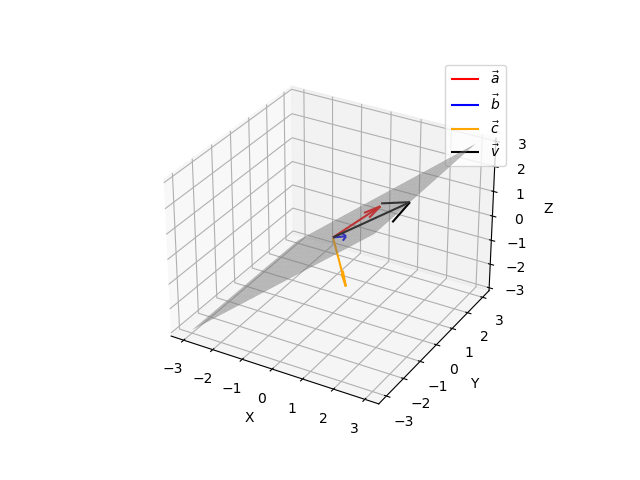
\includegraphics[width=\columnwidth, height=0.8\textheight, keepaspectratio]{Figs/plot(py+C).png}     
\end{frame}

%-------End of Python+C-------------


\begin{frame}[fragile]
    \frametitle{Python Code}
    \begin{lstlisting}

import numpy as np
import matplotlib.pyplot as plt
from mpl_toolkits.mplot3d import Axes3D

u = np.array([1, 1, 1])
v = np.array([1, -1, 1])
w = np.array([3, -1, 3])
x = np.array([1, -1, -1])   

uv = v - u
uw = w - u
normal = np.cross(uv, uw)   
a, b, c = normal
d = 0   


\end{lstlisting}
\end{frame}

\begin{frame}[fragile]
    \frametitle{Python Code}
    \begin{lstlisting}

xx, yy = np.meshgrid(
    np.linspace(-3, 3, 10),
    np.linspace(-3, 3, 10)
)
zz = (-a * xx - b * yy - d) / c

fig = plt.figure()
ax = fig.add_subplot(111, projection='3d')

ax.plot_surface(xx, yy, zz, alpha=0.5, color='grey')


\end{lstlisting}
\end{frame}

\begin{frame}[fragile]
    \frametitle{Python Code}
    \begin{lstlisting}

origin = np.zeros(3)

for vec, color, label in zip([u, v, w, x], ['r', 'g', 'b', 'orange'], [r'$\vec{a}$', r'$\vec{b}$', r'$\vec{v}$', r'$\vec{c}$']):
    ax.quiver(*origin, *vec, color=color, label=label)


ax.set_xlabel('X')
ax.set_ylabel('Y')
ax.set_zlabel('Z')
ax.legend()
plt.savefig("../Figs/plot(py).png")
plt.show()


\end{lstlisting}
\end{frame}


\begin{frame}{Plot-Using Python only}
    \centering
    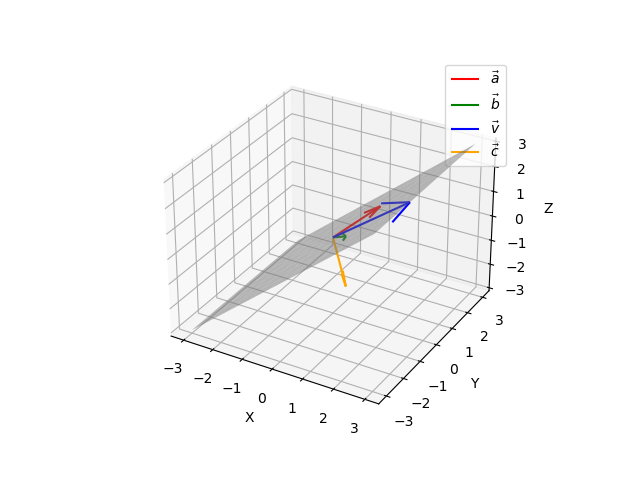
\includegraphics[width=\columnwidth, height=0.8\textheight, keepaspectratio]{Figs/plot(py).png}     
\end{frame}


\end{document}

